The back-end readout card for the system under development, the Zynq UltraScale+ RFSoC ZCU216 Evaluation Card, was chosen taking into consideration the points described in \autoref{sec:selection}.
In this section, the overall architecture and features of the card are presented.
A possibility for evaluation of the card is also demonstrated.
At last, a design for the read-out firmware is proposed. 

\section{Xilinx Zynq UltraScale+ RFSoC ZCU216 Evaluation Card}
Zynq UltraScale+ RFSoCs: Combine RF data converter subsystem and forward error correction with industry-leading
programmable logic and heterogeneous processing capability. Integrated RF-ADCs, RF-DACs, and soft decision FECs (SD-FEC)
provide the key subsystems for multiband, multi-mode cellular radios and cable infrastructure


With the data converters integrated directly into the \gls{fpga} using parallel interfaces, they do not require the
prohibitively high-pin-count external connections needed for discrete parallel interface converters, allowing more converter

\begin{itemize}[noitemsep]
	\item Sixteen 14-bit, 2.5GSPS RF-ADC
	\item Sixteen 14-bit, 10GSPS RF-DAC
	\item I/O expansion options – FPGA Mezzanine Card (FMC+) interfaces, RFMC 2.0 interfaces, and Pmod connections
\end{itemize}
\begin{figure}[tbh]
	\centering
	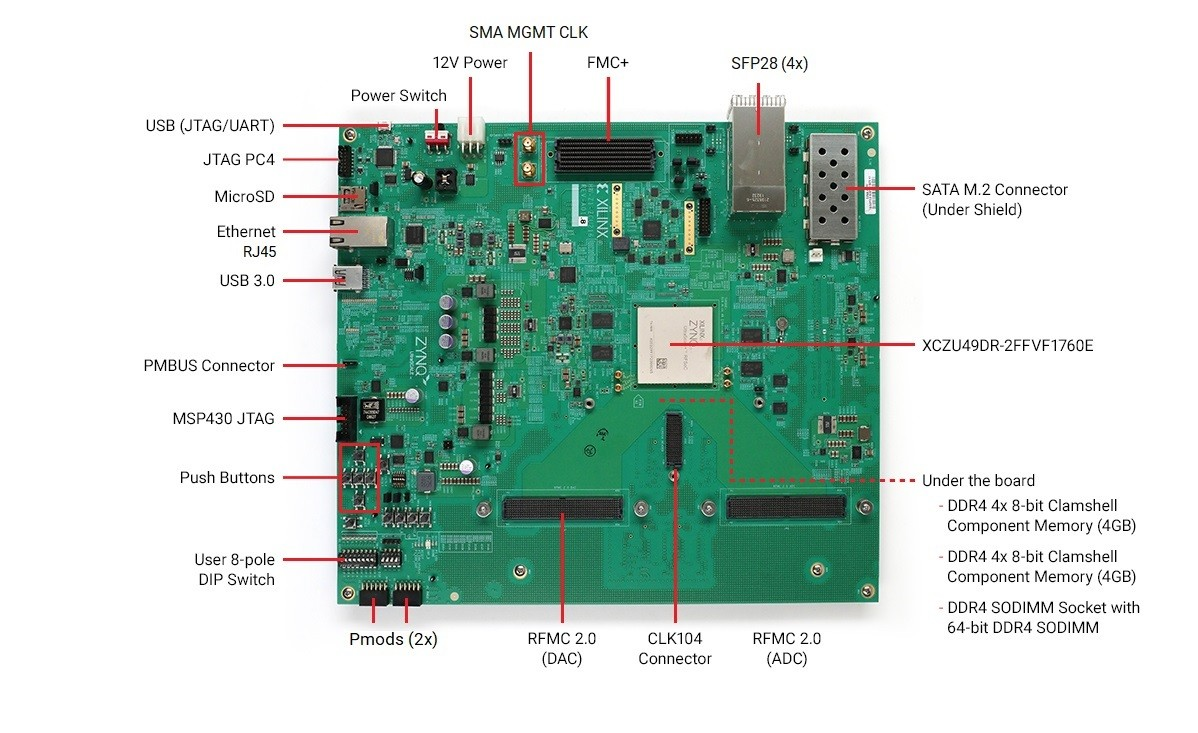
\includegraphics[width = \textwidth]{chap/04-work/img/zcu216}
	\caption{ZCU216 evaluation board}
	\label{fig:zcu216}
\end{figure}

\begin{figure}[tbh]
	\centering
	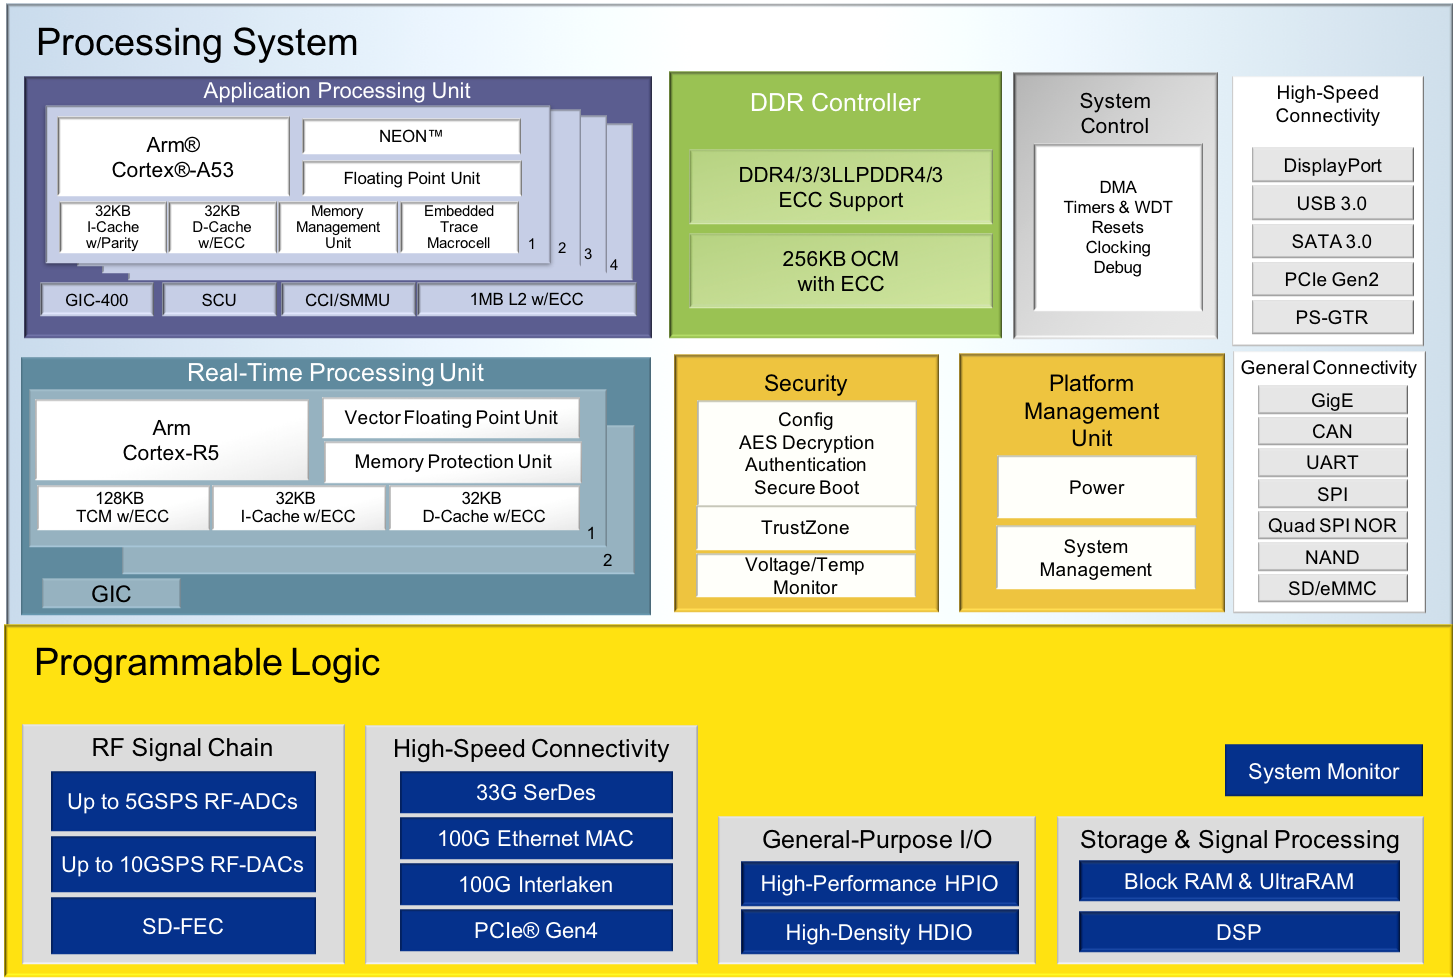
\includegraphics[width = \textwidth]{chap/04-work/img/rfsoc_blockdiagram}
	\caption{RFSoC block diagram}
	\label{fig:rfsoc}
\end{figure}

\section{Features}
\section{Evaluation Tool}

\section{Firmware}
\subsection{RF Data Converter}
\subsection{SoC}
\subsection{RDMA over Converged Ethernet (RoCE)}

\subsection{System Integration}
\paragraph{Interleaving}
The necessary step size for the delay chips, when using 16 \glspl{adc} @\SI{2}{\giga \sample \per \second} in time-interleaving mode, is: $\nicefrac{\SI{2}{\giga \sample \per \second}}{16} = \SI{31}{\pico \second}$
However, providing individual clocks to the \glspl{adc} is not possible on the ZCU216 card. \glspl{adc} are grouped together into tiles, each tile containing four converters. One single reference clock signal is propagated to all tiles. Sampling clock is adjusted at each tile individually, however this clocking signal is the same for all of the four converters in the tile.

Clock to THA: \SI{500}{\mega \hertz}

Total Hold time: \SI{1}{\nano \second}

$\rightarrow$ Step size for delay:
\begin{equation}
\frac{\SI{1}{\nano \second}}{16 \, \text{channels}} = \SI{62.5}{\pico \second}
\end{equation}

